%*******************************************************************
%*******************************************************************
%*******************[       Tipus de Beamer       ]*****************
%*******************************************************************
%*******************************************************************
%*******************************************************************
\documentclass[twocolumn]{beamer}
\DeclareMathAlphabet{\mathpzc}{OT1}{pzc}{m}{it} %
\setbeamertemplate{navigation symbols}{}
\usefonttheme{serif}
\usetheme{Warsaw}
\usepackage{lmodern}% Serveix per que les fonts i altres opcions de LaTeX no donin problemes amb Beamer.
%\beamersetuncovermixins{\opaqueness<1>{25}}{\opaqueness<2->{15}}
%\setbeamercolor{normal text}{bg=blue!20} % Fons en color, no pesa tan com imatge
%\setbeamertemplate{background canvas}{\includegraphics[width=\paperwidth,height=\paperheight]{Fons}}
%*******************************************************************
%*******************************************************************
%*******************[       Classics en català    ]*****************
%*******************************************************************
%*******************************************************************
%*******************************************************************
%Paquets d'idioma i codificació de caràcters
\usepackage[utf8]{inputenc}
\usepackage[T1]{fontenc}
\usepackage[catalan]{babel}

%Paquets d'escriptura matemàtica
\usepackage{amsmath,amsfonts,amssymb,amsthm}

%Definicions,exemples,observacions...
\newtheorem{defi}{Definició}
\newtheorem{exempl}{Exemple}
\newtheorem{obsv}{Observació}
\newtheorem{prop}{Proposició}
\newtheorem{teorm}{Teorema}
\newtheorem{corol}{Corol·lari} 

%Modificacions i noves comandes
\renewcommand\qedsymbol{QED} %Canviem el símbol de demostració final  de un quadrat en blanc a QED 
\newcommand{\R}{\ensuremath{\mathbb{R}}}
\newcommand{\N}{\ensuremath{\mathbb{N}}}
\newcommand{\esp}{\text{ }}

%Altres paquets
\usepackage{enumerate} %Serveix
\usepackage{multirow} %Serveix per agrupar files i columnes
\usepackage{graphicx} %Serveix per introduir imatges
\usepackage{hyperref} %Serveix per que totes les referències que apareguin en el document pdf clicant-hi amb el ratolí, el visor pdf saltarà a la posició referenciada
%\usepackage{enumerate,paralist} %Serveix per ampliar les possibilitats dels entorns de llistes
\usepackage{subfigure} %Serveix per poder generat subfigures.
\usepackage{pstricks-add} %Paquets per a dibuixos amb GeoGebra
\usepackage{centernot} %Serveix taxar coses bé com per exemple $\longrightarrow$ i $\exists$
\usepackage{colortbl} %Serveix per ficar colors a les taules
\usepackage{verbatim}%Serveix per ficar comentaris
\usepackage{booktabs} %Serveix per taules

\usepackage{yhmath}
%Serveix per lletre inicial més elegant i vanidosa
\usepackage{listings}
\usepackage{erewhon}
\usepackage{lipsum}
\usepackage{lettrine}
\usepackage{GoudyIn}
\definecolor{redviolet}{RGB}{52,47,75}
\usepackage{xcolor} 
\renewcommand{\LettrineFontHook}{\color{redviolet}\GoudyInfamily{}}
\setcounter{DefaultLines}{3}%
\usepackage{listings}
% Serveix per ficar caixes
\usepackage{tcolorbox}

%*****************************************************************
%*****************************************************************
%*******************[         El document         ]***************
%*****************************************************************
%*****************************************************************
%*****************************************************************
\begin{document}
\section{Introducció}
\title{\textit{Pla Docent}}
\subtitle{\color{blue!20!black} Taller de Modelització \\ 2n. de Grau en  Matemàtiques \\ \color{black} Universitat Autònoma de Barcelona}
\date{Albert Acebrón, Jaume Betriu, Martina Canet, Marc Graells\\ 13 o 16 de maig de 2019 \\}
\section{Grup 15}
\section{Taller de Modelització}
%Diapositiva 1 (Ens presentem i anunciem el títol)
\begin{frame} 
\maketitle
\centering
\end{frame}
%Diapositiva 2 (Com Esquema)
\begin{frame}{Les quatre parts de la presentació}
\begin{columns}[t]
%c1
\begin{column}{.5\textwidth}
   \setbeamercolor{block title}{use=structure,fg=white,bg=red!75!black}
       \begin{block}{$\blacksquare$ Primera part }
       	\begin{itemize}
       		\small
       		\item $\mathbf{0.}$ Introducció
       		\item $\mathbf{1.}$ Anàlisis del problema \\ $\quad \quad \vdots$
       		\item $\mathbf{5.}$Conclusions
       	\end{itemize}
       \normalsize
       \end{block}
  	\setbeamercolor{block title}{use=structure,fg=white,bg=orange!75!black}
  %>\
  \begin{block}{$\blacksquare$ Tercera part }
  	\begin{itemize}
  		\small
  		\item $\mathbf{3.}$ Model d’Optimització o d’investigació de sistemes
  		\begin{itemize}
  			\footnotesize
  			\item $\mathbf{3.3}$ Biblioteca \textit{subfusions}
  			\item $\mathbf{3.4}$ Resultats i limitacions 
  		\end{itemize}
  	\end{itemize}
  \end{block}
\end{column}
%c2
\begin{column}{.5\textwidth}

    \setbeamercolor{block title}{use=structure,fg=white,bg=green!75!black}
   %>\
   \begin{block}{$\blacksquare$ Segona part }
   	\begin{itemize}
   		\small
   		\item $\mathbf{2.}$ Anàlisis del \textit{Model actual}
   		\begin{itemize}
   			\footnotesize
   			\item $\mathbf{2.1 \text{ i } 2.2}$ Dades obtingudes i facilitades
   			\item $\mathbf{2.3}$ Algunes curiositats 
   			\item $\mathbf{2.4 \text{ i } 2.5}$ Anàlisis  i Conclusions
   		\end{itemize}
   	\end{itemize}
   	\normalsize
   \end{block}
   \setbeamercolor{block title}{use=structure,fg=white,bg=cyan!75!black}
   %>\
       \begin{block}{$\blacksquare$ Quarta part}
       	\begin{itemize}
       		\small
       		\item $\mathbf{4.}$ \textit{Model/Mètode} $\times$ Subhastes
       		\begin{itemize}
       			\footnotesize
       			\item $\mathbf{4.2}$ Model \textit{Kiwis}
       			\item $\mathbf{4.3}$ Altres Models 
       		\end{itemize}
       	\end{itemize}
       \end{block}
\end{column}
\end{columns}
\end{frame}
%
%Diapositiva 3 (1.)
\begin{frame}{$\mathbf{1.}$ Anàlisis del problema}
\begin{columns}[t]
	%c1
\begin{column}{.5\textwidth}
	\setbeamercolor{block title}{use=structure,fg=white,bg=red!75!black}
	%>\
	\begin{block}{Enunciat del problema, \textbf{part 1}}
		\small
		\textit{{\color{cyan!60}$\blacksquare$}$^{(01)}${\color{black!80}Un departament d'una universitat té diferents tasques docents assignades, que s'han de repartir entre els seus professors.}}
		
		\textit{{\color{blue!60}$\blacksquare$}$^{(02)}$ Actualment es distribueixen segons les hores de classe de cada tasca. Se suposa que el nombre d'hores mesura l'esforç associat a una tasca, però en la pràctica això no és prou realista, la qual cosa genera desequilibris.}
	\end{block}
\end{column}
\begin{column}{.5\textwidth}
\setbeamercolor{block title}{use=structure,fg=white,bg=red!75!black}
%>\
\begin{block}{Enunciat del problema, \textbf{part 2}}
	\small	
	 \textit{{\color{green!60}$\blacksquare$}$^{(03)}$ {\color{black!80}Es tracta de trobar un mètode més equilibrat per valorar les tasques docents, que tingui en compte la demanda per cada tasca per part dels diferents professors.}}
	 
	\textit{{\color{purple!60}$\blacksquare$}$^{(04)}$Es podria expressar aquesta demanda a través d'una mena de subhasta.}
	
	\textit{{\color{violet!60}$\blacksquare$}$^{(05)}${\color{black!80}S'haurien de tenir en compte algunes restriccions, com per exemple, que tothom faci la mateixa quantitat de docència o la restricció que hi hagi a cada departament.}}
\end{block}
\end{column}
\end{columns}
\end{frame}
%Diapositiva 4 (1.)
\begin{frame}
\setbeamercolor{block title}{use=structure,fg=white,bg=red!75!black}
%>\
\begin{block}{Anàlisis Enunciat}
\begin{itemize}
	\footnotesize
	\item[{ \color{cyan!60} \underline{\underline{\normalcolor (01)}}}] El problema abstracte consisteix en una tasca de repartiment o assignació. Concretament, els \textbf{objectes a repartir} són les tasques docents que han de ser repartides entre  el professorat, cada possible assignació s'anomenarà \textbf{pla docent} o \textbf{solució} de forma anàloga en funció del context.\\
	\item[{ \color{blue!60} \underline{\underline{\normalcolor (02)}}}] Acceptem que el \textit{Model actual} genera solucions \textbf{subòptimes} i això ho  justificarem amb els mateixos arguments del enunciat.\\
	\item[{ \color{green!60} \underline{\underline{\normalcolor (03)}}}] Es requereix { \color{green!60} \underline{\normalcolor mètode}} per { \color{green!60} \underline{\normalcolor valorar}} i { \color{green!60} \underline{\normalcolor repartir}} tasca docent en funció de la demanda del professorat. A més ha de poder aportar una solució millor \footnote{Equivalentment menys desequilibrada.}. 
	\item[{ \color{purple!60} \underline{\underline{\normalcolor (04)}}}] Es proposa com a \textbf{alternativa}  desenvolupar un  { \color{purple!60} \underline{\normalcolor mètode basat en subhasta}}.
	\item[{ \color{violet!60} \underline{\underline{\normalcolor (05)}}}] S'expressa anticipadament que el \textbf{model/mètode} ha de tenir \textbf{restriccions}  i s'expliciten dos de necessàries. El volum del treball ha de ser \textit{homogeni}\footnote{Entesa com la qualitat de: quantitat de docències semblants entre el professorat.}. El mètode ha de contemplar la possibilitat de restriccions pròpies del departament. 
\end{itemize}
\end{block}
\end{frame}
%Diapositiva 5 (2.)
\begin{frame}{$\mathbf 2.$ Anàlisis del \textit{Model Actual}}
\begin{columns}[t]
	%c1
	\begin{column}{.5\textwidth}
		 \setbeamercolor{block title}{use=structure,fg=white,bg=green!75!black}
		%>\
		\begin{block}{Alguns detalls:}
			\begin{itemize}
				\footnotesize
				\item 3 graus propis + 26 graus externs. \\ \textit{\footnotesize \color{blue} 500 sol·licituds $\approx$ 150 assignatures}
				\item 5 subdepartaments del departament. \\ \textit{ \footnotesize \color{blue} Assignatures 3r i 4rt graus propis.}
				\item  Ja ve fixat el horari, nombre de alumnes i la tipologia. \\ \textit{\footnotesize \color{blue} Això és si és una classe de problemes o de seminaris o $\cdots$}
				\item Les assignatures \textbf{només} són comptades per hores de classe realitzades.
			\end{itemize}
		\end{block}
	\end{column}
	%c2
	\begin{column}{.5\textwidth}
		\setbeamercolor{block title}{use=structure,fg=white,bg=green!75!black}
		
		\begin{block}{\Large$\sum:   $}
			\begin{itemize}
			\footnotesize
			\item El nombre de hores que fa cada professor pot ser molt diferent. \\ \textit{\footnotesize \color{blue} oscil·la entre 60 i 240 hores per any}
			\item Actualment el model intenta minimitzar:
			\textit{\footnotesize \color{blue}
				\\-Dispersió:$$\sum_{i=0}^{112} a_{i}$$
				\\-Deute personal o Saldo}
		     \end{itemize}
		\end{block}
	
		\Huge$\quad  \quad  \quad \cdots$ 
		
	    \end{column}
\end{columns}
\end{frame}


%Diapositiva 6 (2.)
\begin{frame}{Resultats \textit{Model Actual}, valors numèrics }\setbeamercolor{block title}{use=structure,fg=white,bg=green!75!black}

\begin{block}{Dades del \textit{Model actual}}
	\begin{itemize}
		\item El $\sum$ de saldos positius és \texttt{1793} hores.	
		\item El $\sum$ de saldos negatius és \texttt{-2671.0} hores.	
		\item El $\sum$ de saldos positius i negatius  és \texttt{-1122} hores, que és un \texttt{\textbf{8.968825 \%}} del nombre d'hores total que haurien de fer tots els professors.
		\item La mitjana aritmètica d' assignatures que fa cada professor és de  $\approx 5. \wideparen{972}$. 
	\end{itemize}
\end{block}
\end{frame}





%Diapositiva 6 (2.)
\begin{frame}{Resultats \textit{Model Actual}, gràfics}
\begin{figure}
	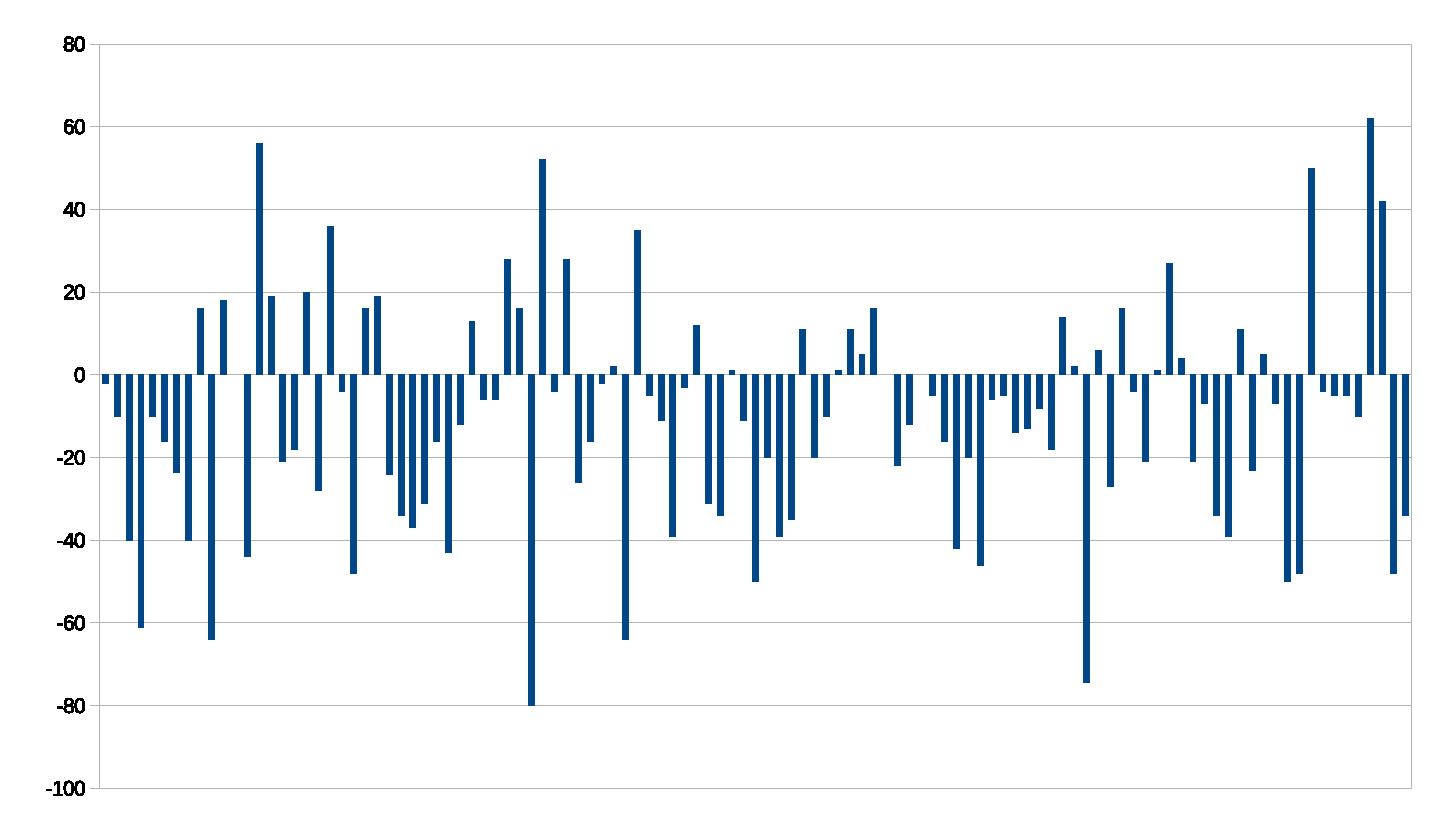
\includegraphics[width=10cm]{saldo_actual}
	\caption{Saldos \texttt{TOTAL} actual del professorat any 2018}
\end{figure}
\end{frame}


%Diapositiva 6 (2.)
\begin{frame}{Resultats \textit{Model Actual}, gràfics}
\begin{figure}
	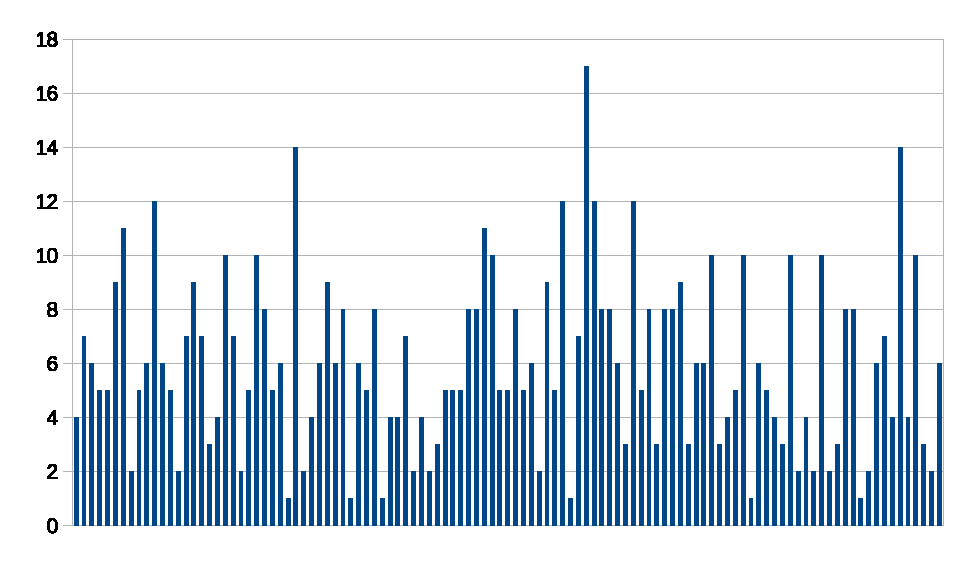
\includegraphics[width=10cm]{dispersio_actual}
	\caption{Dispersió \texttt{TOTAL} actual del professorat any 2018}
\end{figure}
\end{frame}


%Diapositiva 7 (2.)
\begin{frame}{$\mathbf 2.$ Conclusions del \textit{Model Actual}}
\begin{columns}[t]
	%c1
	\begin{column}{.5\textwidth}
		\setbeamercolor{block title}{use=structure,fg=white,bg=green!75!black}
		%>\
		\begin{block}{Conclusions anàlisis}
			\begin{itemize}
				\item Variància molt alta.
				\item Requereix \textit{alt grau} de dedicació.
			\end{itemize}
		\end{block}
	\end{column}
	%c2
	\begin{column}{.5\textwidth}
\begin{figure}
	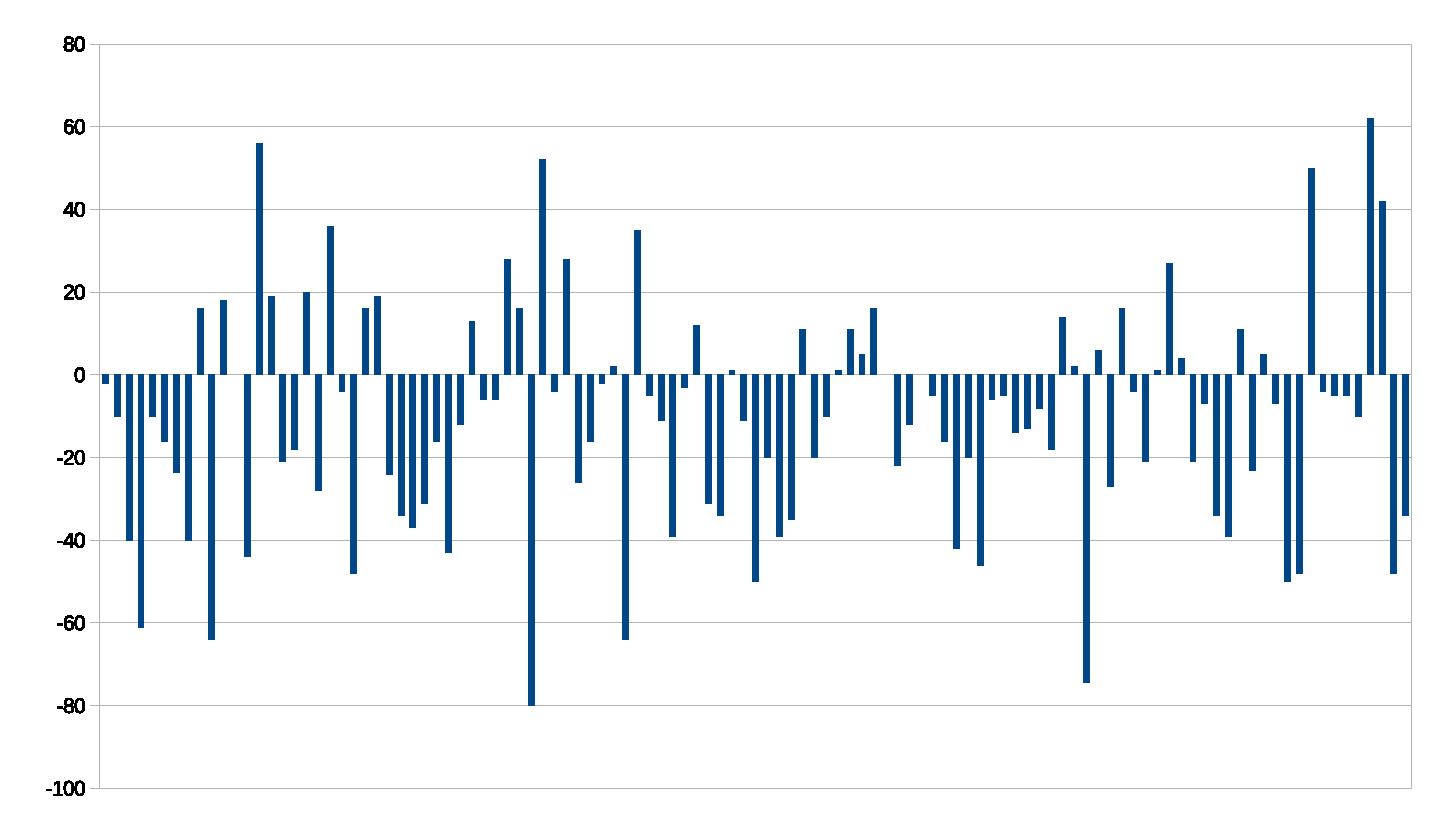
\includegraphics[width=5cm]{saldo_actual}
	\caption{Saldos \texttt{TOTAL} actual del professorat any 2018}
\end{figure}
	\end{column}
\end{columns}
\end{frame}

%Diapositiva 10 (3.)
\begin{frame}{$\mathbf 3.$ Model d’Optimització o d’investigació de sistemes}
\begin{columns}[t]
%c1
\begin{column}{.5\textwidth}
	\setbeamercolor{block title}{use=structure,fg=white,bg=orange!75!black}
	%>\
	\begin{block}{Una noció del model}
		La gràcia està en escollir uns \emph{criteris raonables}
		a partir dels quals , i donades unes \textbf{restriccions}, definir una \textbf{funció objectiu} a optimitzar.
	\end{block}
\setbeamercolor{block title}{use=structure,fg=white,bg=orange!75!black}

\begin{block}{Optimització}
\texttt{\textbf{maximitzar} o \textbf{minimitzar}} \texttt{f}
\\ 
\texttt{Subjecte a}
\\
$\quad $ \texttt{\textbf{restriccions}}
\end{block}
\end{column}
%c2
\begin{column}{.5\textwidth}
\begin{figure}
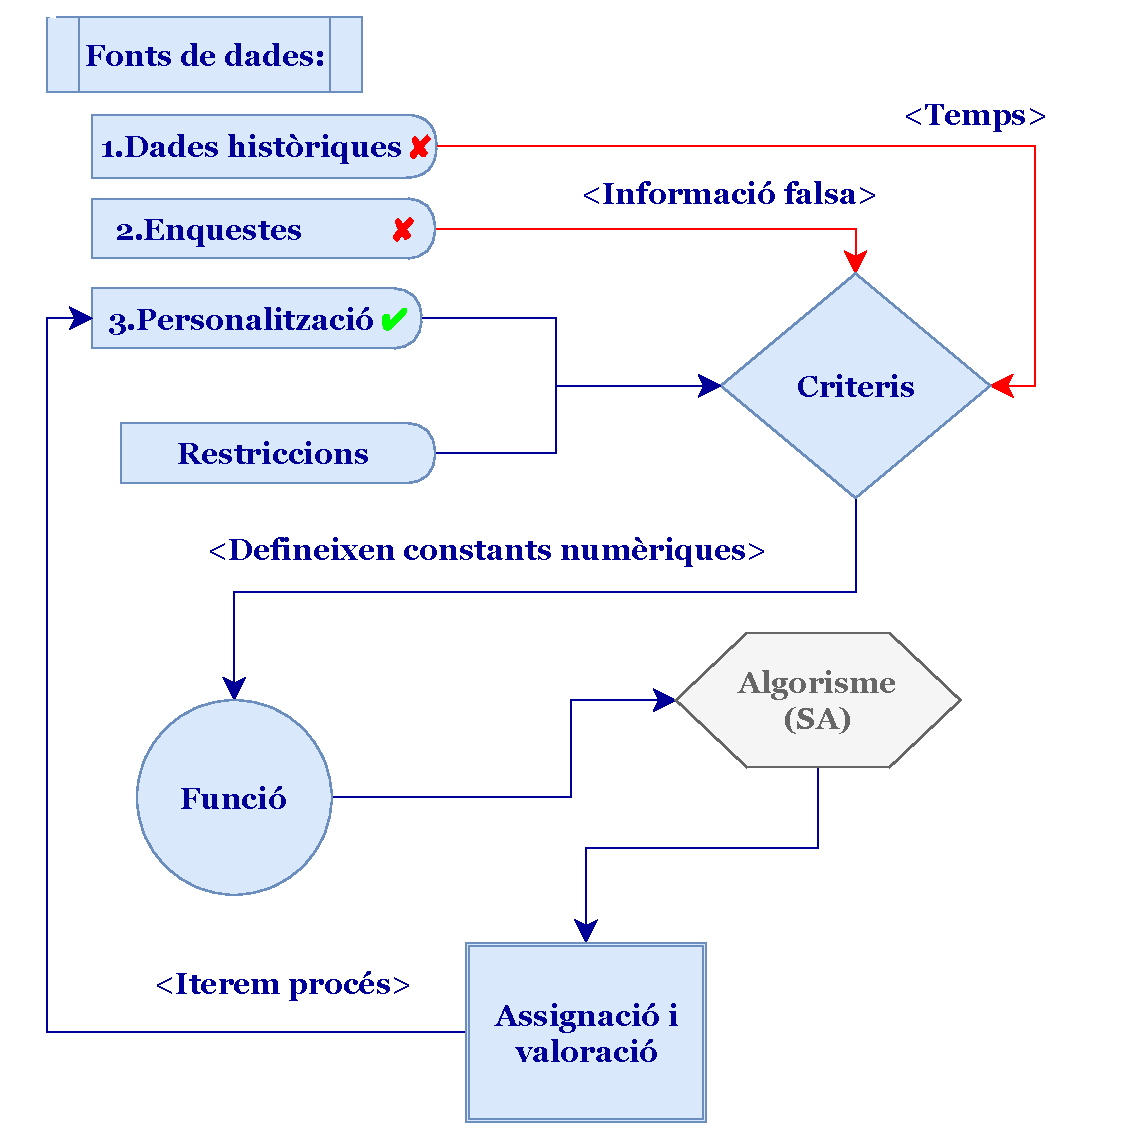
\includegraphics[width=6cm]{algor}
\end{figure}
\end{column}
\end{columns}
\end{frame}



%Diapositiva 10 (3.)
\begin{frame}{\textit{Biblioteca} de funcions i restriccions}
\begin{columns}[t]
	%c1
	\begin{column}{.5\textwidth}
		\setbeamercolor{block title}{use=structure,fg=white,bg=orange!75!black}
		%>\
		\begin{block}{Funció de objectiu $F(a)$}
		\begin{itemize}
		 \item Com \textbf{modelitzem} aquest criteris?
		 \item Potser seria interessant donar una \textbf{Biblioteca} de subfusions i \text{restriccions}.
		\end{itemize}
		\end{block}
		\setbeamercolor{block title}{use=structure,fg=white,bg=orange!75!black}
		
		\begin{block}{Funció com a $\sum$ de \textit{funcions}}
			
			\texttt{\color{green!75!black!75}def:} \texttt{\textbf{func1({\color{blue!75!black!75}a}), func2({\color{blue!75!black!75}a}),.. }}
			\\
			$\quad$\texttt{\color{purple!75!black!75}\textbf{minimitzar}}( \texttt{F({\color{blue!75!black!75}a})})
			\\ 	
			$\quad$ \texttt{\color{red!75!black!75}subj }: \texttt{rst1, rst2, ...}
			\\
		\end{block}
	\end{column}
	%c2
	\begin{column}{.5\textwidth}
		\setbeamercolor{block title}{use=structure,fg=white,bg=orange!75!black}
		\begin{block}{Un esquema}
		\begin{itemize}
		 \item Sigui $a \in \mathbb{A}$ on $|\mathbb{A}|\approx10^{5000}$ conjunt de les possibles assignacions (\textbf{solucions}).
		 \item Llavors volem trobar $a_{\sim opt} \in \mathbb{A}$
		 tal que $F(a_{\sim opt})$ sigui prou petit.
		 \item Donem exemples de \texttt{\textbf{func1({\color{blue!75!black!75}a}), func2({\color{blue!75!black!75}a}),.. }}
		  \end{itemize}
		\end{block}
	\end{column}
\end{columns}
\end{frame}



\begin{frame}{\textit{Biblioteca} de funcions i restriccions}
\begin{figure}
	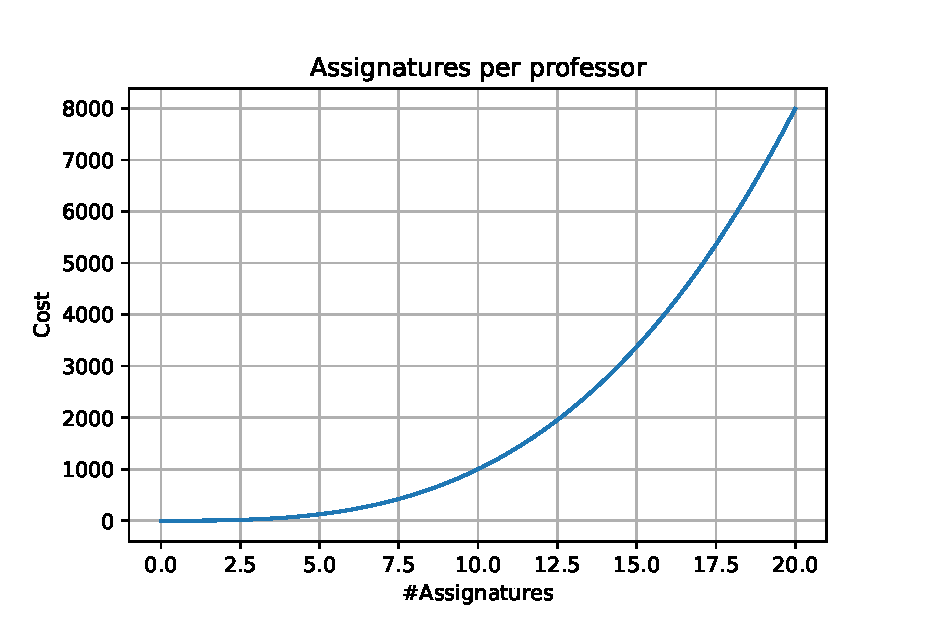
\includegraphics[width=9cm]{Assignatures}
	\caption{$x^3$}
\end{figure}
\end{frame}

\begin{frame}{\textit{Biblioteca} de funcions i restriccions}
\begin{figure}
	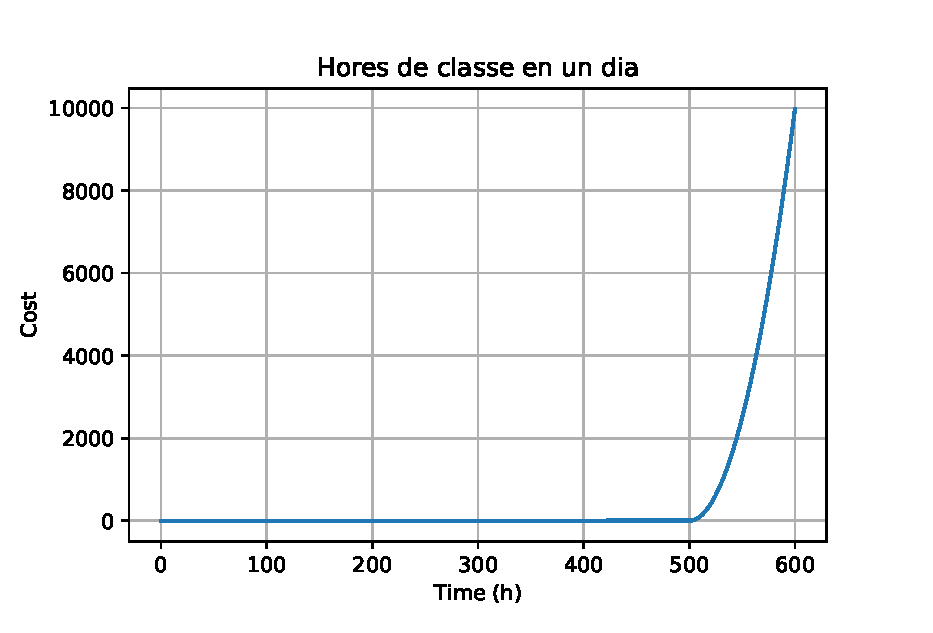
\includegraphics[width=8.5cm]{hores_dia}
	\caption{
	$f(x):=\left\lbrace 
	\begin{matrix}
		(x-500)^2& \text{ si}& x>500\text{ ,} \\
		0& \text{ si}& x\leq 500& \end{matrix}
	\right.$
	}
\end{figure}
\end{frame}

\begin{frame}{\textit{Biblioteca} de funcions i restriccions}
\begin{figure}
	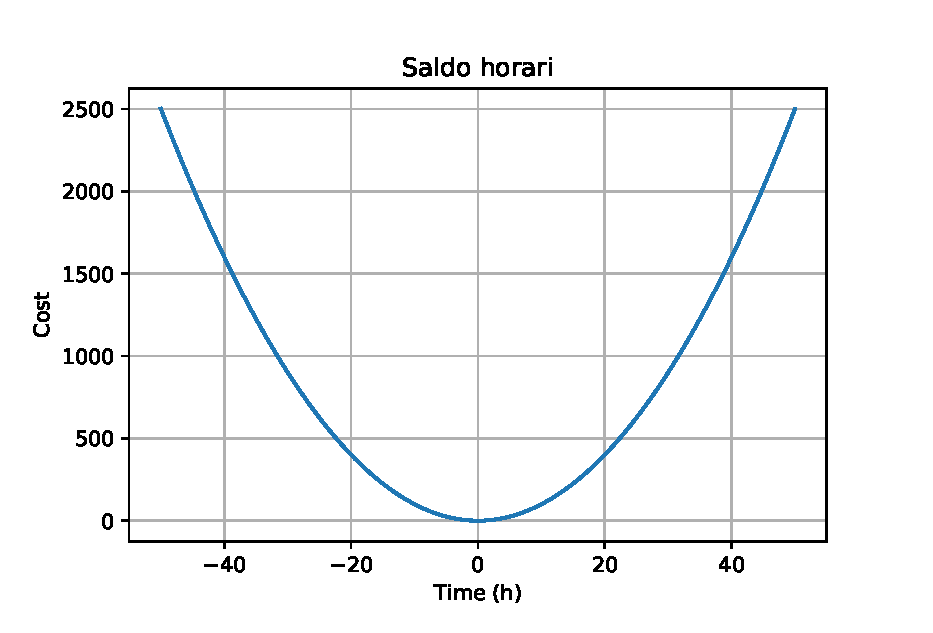
\includegraphics[width=9cm]{saldo}
	\caption{$x^2$}
\end{figure}
\end{frame}
\begin{frame}{\textit{Biblioteca} de funcions i restriccions}
\begin{figure}
	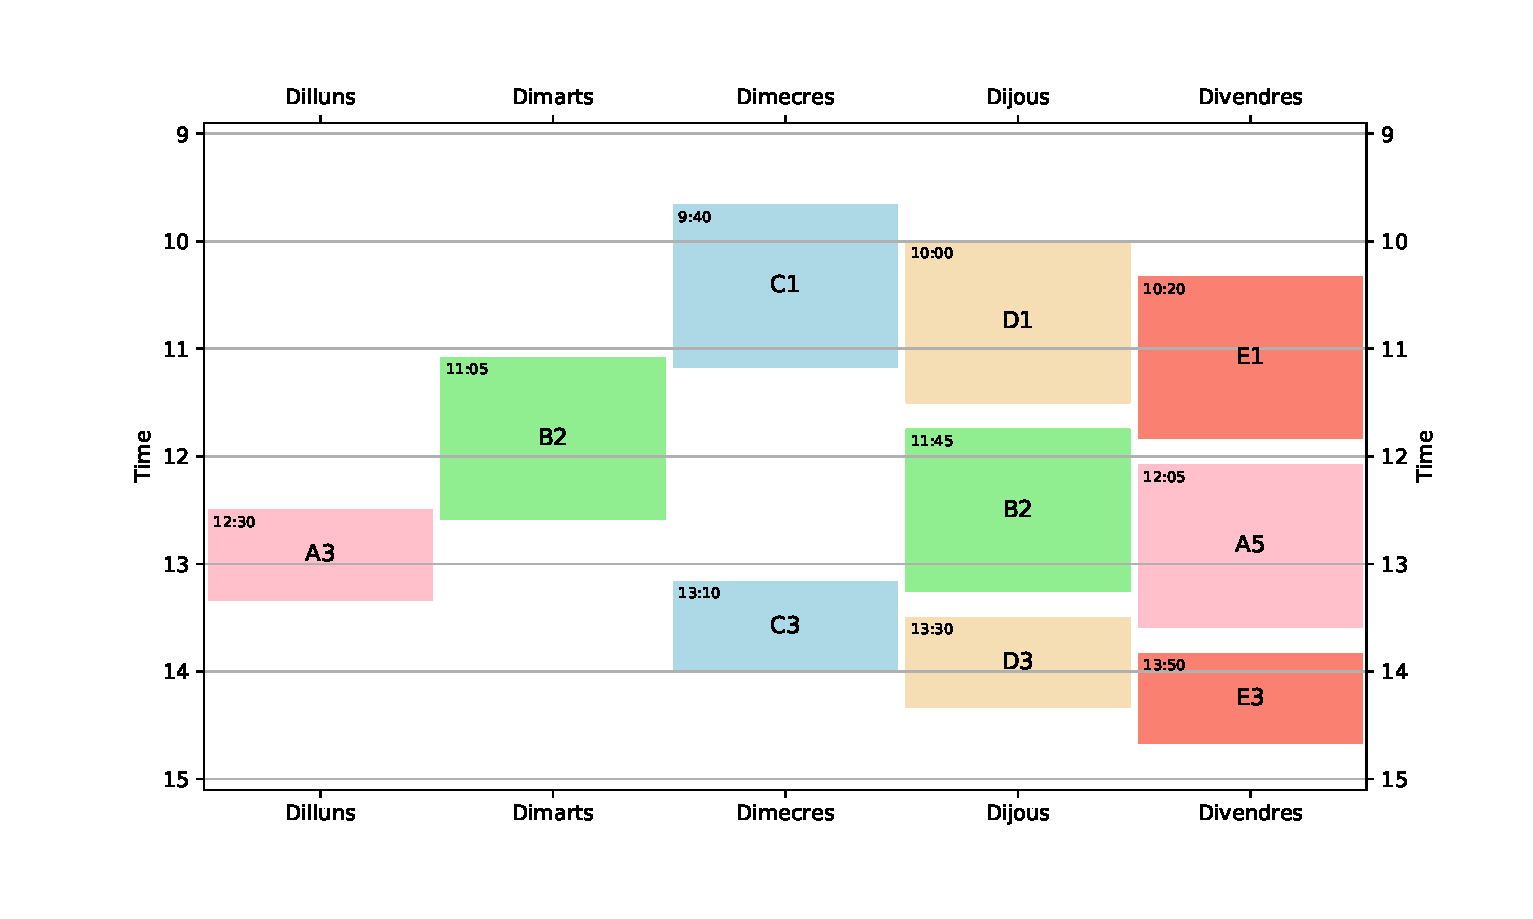
\includegraphics[width=9cm]{../PD_Plots/llibreria_funcs/horari}
	\caption{La distància entre classes es calcula entre dies}
\end{figure}
\end{frame}

\begin{frame}{\textit{Biblioteca} de funcions i restriccions}
\begin{figure}
	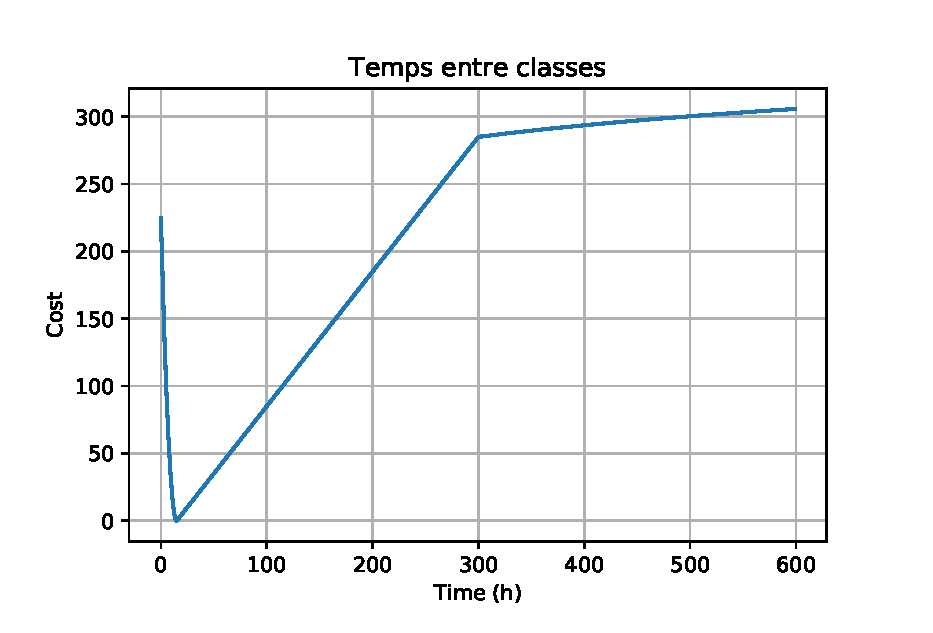
\includegraphics[width=9cm]{interclass}
	\caption{$x^2$, $x$ i $log(x)$}
\end{figure}
\end{frame}


%Diapositiva 10 (3.)
\begin{frame}{Resultats i limitacions del mode}
\begin{columns}[t]
	%c1
	\begin{column}{.5\textwidth}
		\setbeamercolor{block title}{use=structure,fg=white,bg=orange!75!black}
		%>\
		\begin{block}{Limitacions}
			Malgrat que l'\textbf{espai de solucions} és finit, com que la seva \textbf{dimensió} és $|\mathbb{A}|\approx10^{5000}$ no podem  garantir que la millor assignació que trobem és correspongui amb un  \textbf{mínim} de la \textbf{funció objectiu}. 
			I \textit{a priori} tampoc podem donar cap altra garantia sobre la \textit{qualitat} de la solució a la que arribaran els \textit{algorismes} d'optimització.
		\end{block}
		\setbeamercolor{block title}{use=structure,fg=white,bg=orange!75!black}
		
	\end{column}
	%c2
	\begin{column}{.5\textwidth}
		\setbeamercolor{block title}{use=structure,fg=white,bg=orange!75!black}
		
		\begin{block}{Justificació}
			\begin{itemize}
				\item \textbf{Solució factible}
				\item \textbf{Solució bona} ja que millora anys anterior.
			\end{itemize}
		\end{block}
		\begin{block}{Conclusions i resultats}
			A partir de simulacions concloem que les solucions que trobem  \textbf{milloren} les obtingudes amb el \textit{model actual}, respecte els aspectes que és volen a \textbf{optimitzar}.
		\end{block}
	\end{column}
\end{columns}
\end{frame}
\begin{frame}{Conclusions Model d'investigació de sistemes}
\begin{figure}
	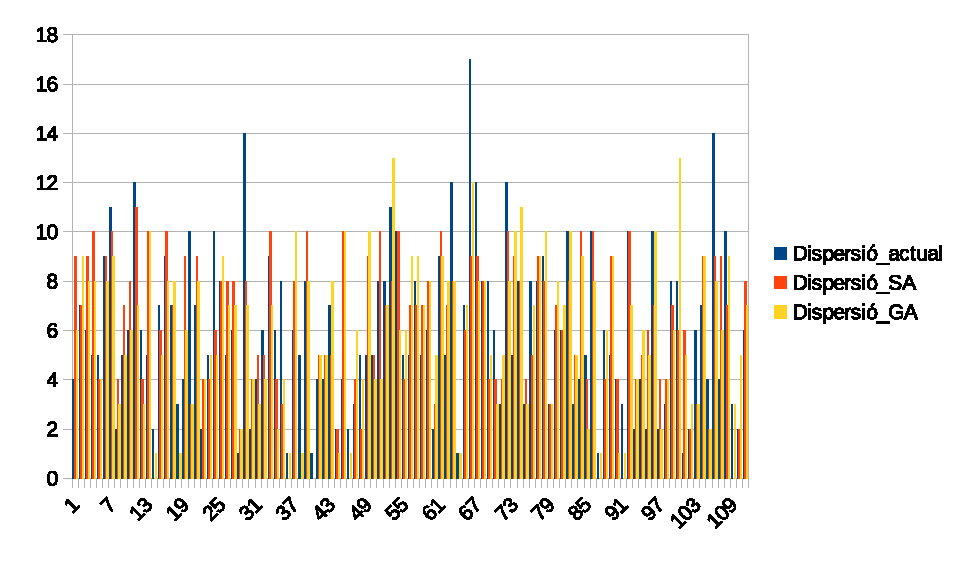
\includegraphics[width=9cm]{dispersio_diff_ga}
	\caption{Dispersió d'assignatures per professor}
\end{figure}
\end{frame}

\begin{frame}{Conclusions Model d'investigació de sistemes}
\begin{figure}
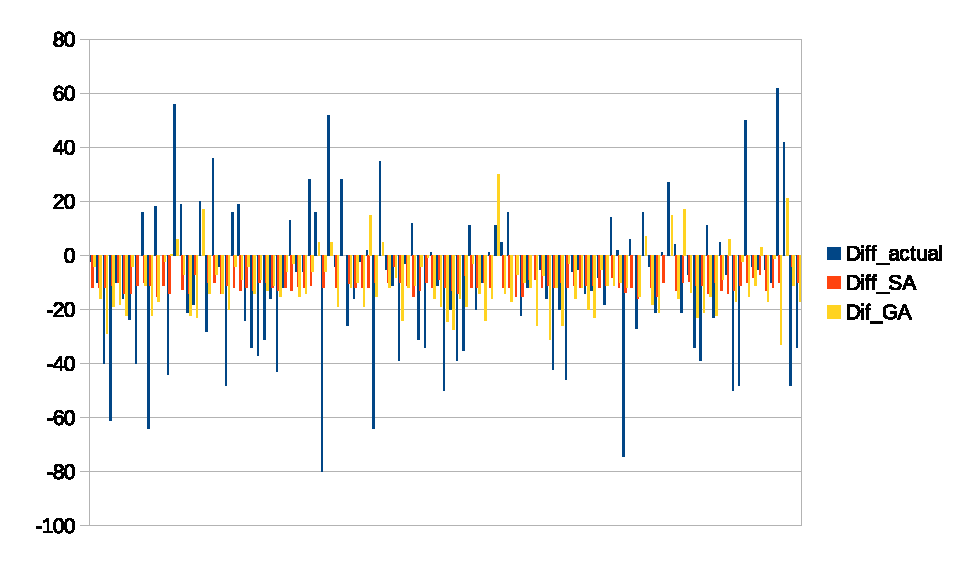
\includegraphics[width=9cm]{saldo_diff_ga}
\begin{tabular}{c|c|c}
	\textbf{Model} & \textbf{Actual} & \textbf{Funció (SA)} \\
	Variància & 737.0676 & 14.7221 \\
	Suma absoluta & 2498 & 1156 \\
\end{tabular}
\end{figure}
\end{frame}

%Diapositiva 11 (3.)
\begin{frame}{Problemàtiques i beneficis de les Subhastes}
\begin{columns}[t]
	%c1
	\begin{column}{.3\textwidth}
		\setbeamercolor{block title}{use=structure,fg=white,bg=cyan!75!black}
		%>\
		\begin{block}{Problemàtiques}
			\begin{itemize}
				\item Concurrència
				\item Incentius han d'estar ben alineats
			\end{itemize}
		\end{block}
		\setbeamercolor{block title}{use=structure,fg=white,bg=cyan!75!black}
		%>\
		
		\begin{block}{Beneficis}
			\begin{itemize}
				\item Transparència
				\item Simplicitat
			\end{itemize}
		\end{block}
	\end{column}
	%c2
	\begin{column}{.7\textwidth}
		
		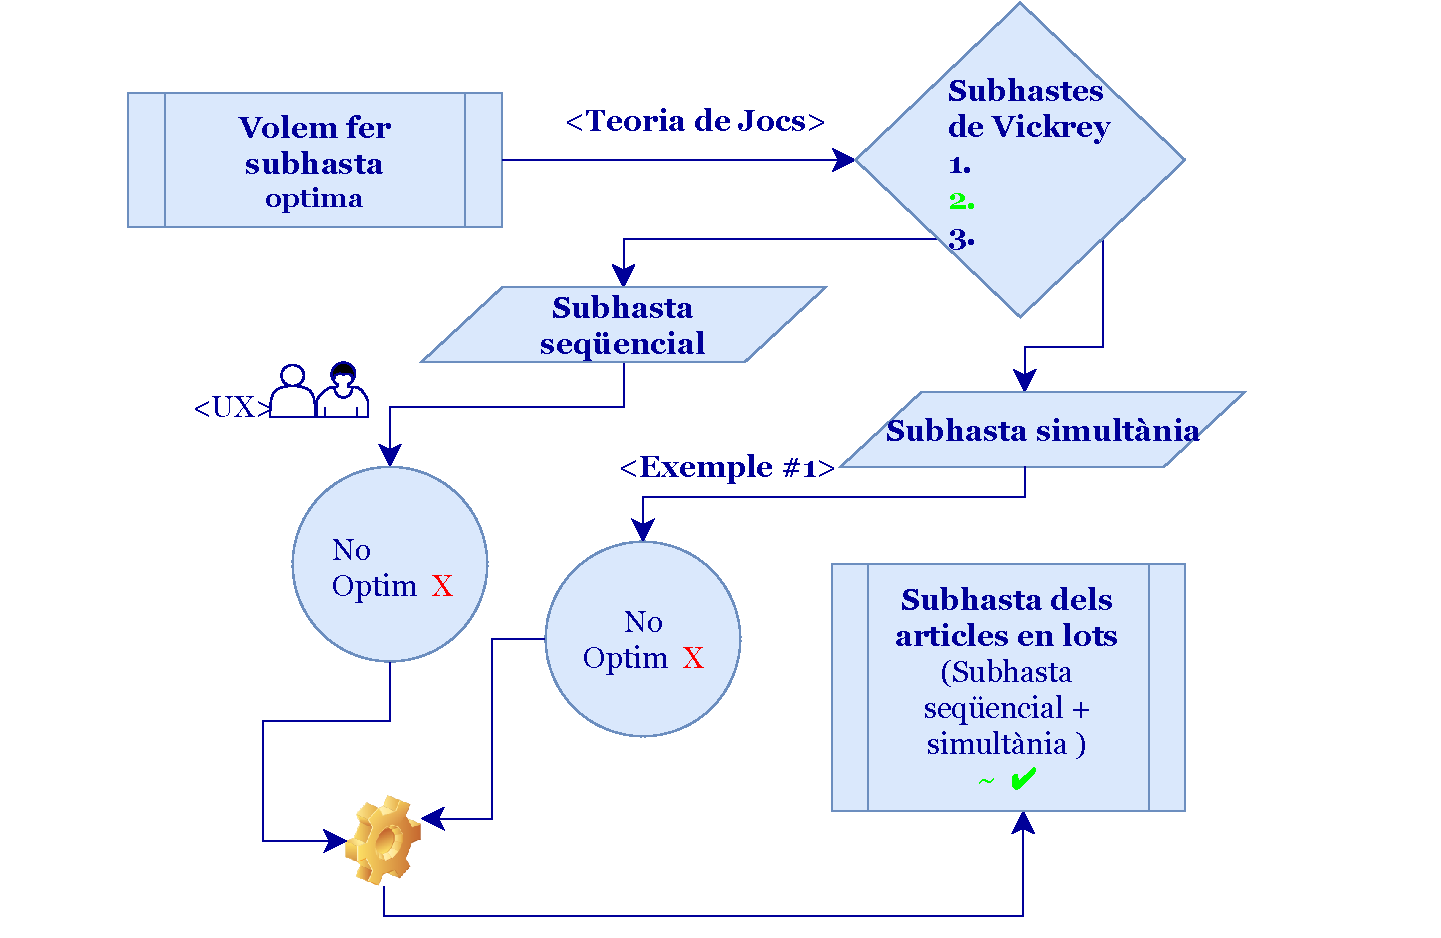
\includegraphics[width=9cm]{subs}	 
		
	\end{column}
\end{columns}
\end{frame}

\iffalse
%Diapositiva 11 (3.)
\begin{frame}{$\mathbf 4.$ \textit{Models} o \textit{Mètodes} per Subhastes}
\begin{columns}[t]
	%c1
	\begin{column}{.5\textwidth}
		\setbeamercolor{block title}{use=structure,fg=white,bg=cyan!75!black}
		%>\
		\begin{block}{Estat del model}
			Lorem ipsum dolor sit amet,
			consectetuer adipiscing elit. Upurus elit, vestibulum ut,
			placerat ac, adipiscing vitae,
			felis. Curabitur dictum gravida
			mauris. Nam arcu libero,
			nonummy eget, consectetuer ivulputate a, magna. Donec
			vehicula augue eu neque.
		\end{block}
	\end{column}
	%c2
	\begin{column}{.5\textwidth}
		\setbeamercolor{block title}{use=structure,fg=white,bg=cyan!75!black}
		\begin{block}{Valors rellevants}
			Lorem ipsum dolor sit amet,
			adipiscing elit. Upurus elit, vestibu
			consectetuer ok
		\end{block}
		
\includegraphics[width=3.5cm]{eps}
	\end{column}
\end{columns}
\end{frame}
\fi

%Diapositiva 11 (3.)
\begin{frame}{Model $Kiwis$}
\begin{columns}[t]
	%c1
	\begin{column}{.5\textwidth}
		\setbeamercolor{block title}{use=structure,fg=white,bg=cyan!75!black}
		%>\
		\begin{block}{1.Repartiment $Kiwis$}
			\begin{itemize}
				\item Subhastes basades en moneda de canvi ($Kiwis$)
				\item Es parteix de 10 $Kiwis$
				\item +5 $Kiwis$ per cada 10 hores de saldo positiu
				\item A partir del segon any:
			\end{itemize}
		\end{block}
	\end{column}
	%c2
	\begin{column}{.5\textwidth}
		\setbeamercolor{block title}{use=structure,fg=white,bg=cyan!75!black}
		\begin{block}{A partir del segon any:}
			\begin{itemize}
				\footnotesize
				\item + $X$ kiwis per $X$ assignatures no triades pel professor
				\item +30 kiwis per un 4.5 o més en les enquestes
			\end{itemize}
		\end{block}
	\begin{figure}
		\centering
		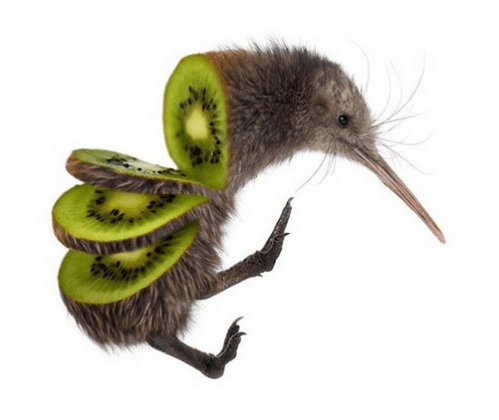
\includegraphics[width=3.5cm]{kiwi}
	\end{figure}
	\end{column}
\end{columns}
\end{frame}

\begin{frame}{Funcionament $Kiwis$}
\setbeamercolor{block title}{use=structure,fg=white,bg=cyan!75!black}
\begin{block}{1.Repartiment $Kiwis$}
\begin{itemize}
	\item Subhasta en blocs mitjançant pdf (evitant bloqueig)
	\item Valor inicial 0, puja mínima 1
	\item Atorguem les assig. al millor postor
	\item Empat $\Rightarrow$ guanya qui té més kiwis al inici
	\begin{itemize}
		\item Si empatem novament revaloritzem amb valor de mercat i la subhastem a la següent
		\item Ultima subhasta: possibilitat de fer pujes negatives
	\end{itemize}
\end{itemize}
\end{block}
\end{frame}


\begin{frame}{Funcionament $Kiwis$}
\setbeamercolor{block title}{use=structure,fg=white,bg=cyan!75!black}
\begin{block}{Revalorització de les hores}
\begin{itemize}
\item Valor assig. $=$ h inicialment
\item Valor final $$h'=h-\frac{num.profs.que.han.pujat}{num.profs.que.han.pujat+1}-\frac{preu.en.Kiwis}{preu.en.Kiwis+1}$$
\item Assignatures no assignades o assignades per $\leq0$ kiwis  $h’=h+1$
\item Assignatures sense pujes repartides per $f(x)$ als prof. $\leq \frac{2M}{3}$
\end{itemize}
\end{block}
\end{frame}

%Diapositiva 6 (2.)
\begin{frame}{Definició de subhasta òptima}\setbeamercolor{block title}{use=structure,fg=white,bg=cyan!75!black}

\begin{block}{Subhastes òptimes}
	\begin{itemize}
		\item Hi ha una branca sencera (Auction theory) de l'Economia que es dedica a l'estudi de subhastes. De manera que hi ha molta recerca sobre com evaluar-les.
		\item Definició: Una subhasta és òptima si el sistema maximitza l'utilitat de tots els participants, en el nostre cas això passa si el sistema obté el màxim (mínim) en pujes a l'alta (baixa).
	\end{itemize}
\end{block}
\end{frame}

\begin{frame}{Problemes}\setbeamercolor{block title}{use=structure,fg=white,bg=cyan!75!black}
\begin{block}{Problemes en subhastes no òptimes}
	\begin{itemize}
		\item Subhastes parcialment simultànies porten a ineficiencies causades pel bloqueig de moneda.
		\item Subhastes simples no funcionen bé en el cas en que hi hagin dependències entre puges (ex: només vull aquesta assignatura si tinc aquesta altra assignatura).	
		\item Cas concret: Un professor vol fer totes les seves assignatures en un només 2 dies de la setmana.
		\item Si els actors tenen que especular el model de subhasta no serà òptim, volem evitar la especulació.
		\item Com assignem les assignatures que no vol ningú?
	\end{itemize}
\end{block}
\end{frame}

\begin{frame}{Solució}\setbeamercolor{block title}{use=structure,fg=white,bg=cyan!75!black}
\begin{block}{Model de subhastes}
	\begin{itemize}
		\item Subhastes a la baixa per hores (en kiwis funcionaria igualment).
		\item De vickrey (en cas de tenir pujes a la baixa fiquem un màxim superior).
		\item Combinatorials.
		\item Totalment simùltanies/paral·leles.
	\end{itemize}
\end{block}
\end{frame}

\begin{frame}{El gran problema}\setbeamercolor{block title}{use=structure,fg=white,bg=cyan!75!black}
\begin{block}{El problema del guanyador en subhastes combinatorials}
	\begin{itemize}
		\item Les subhastes combinatorials han estat molt estudiades a la literatura.
		\item Està demostrat que el problema de trobar els guanyadors d'aquest tipus d'apostes es NP-Complet, de manera que no el podem resoldre en un temps tractable ja que la complexitat és massa alta.
	\end{itemize}
\end{block}
\end{frame}

\begin{frame}{La gran solució}\setbeamercolor{block title}{use=structure,fg=white,bg=cyan!75!black}
\begin{block}{Transformació}
	\begin{itemize}
		\item Transformem el problema a un de pujes condicionals (puja A només es vàlida si la puja B és guanyadora).
		\item Podem donar un algoritme que ens permet transformar un problema en l'altre en temps polinomial de manera que demostrem que els dos problemes són equivalents.
	\end{itemize}
\end{block}
\begin{block}{Algoritme per decidir guanyador en el nou problema}
	\begin{itemize}
		\small
		\item Assumim que totes les pujes són vàlides. Si alguna puja guanyadora depèn d'una perdedora, invalidem la guanyadora i la segona passa a ser la guanyadora.
		\item La persona que ha guanyat més pujes tria les assignatures que vol (de forma polinòmica).
		\item Tornar al pas 1.
	\end{itemize}
\end{block}
\end{frame}

\begin{frame}{Anàlisis de l'algoritme}\setbeamercolor{block title}{use=structure,fg=white,bg=cyan!75!black}
\begin{block}{Complexitat}
	\begin{itemize}
		\item L'algoritme és NP, però si en el moment de crear noves pujes restringim la profunditat màxima de cadenes condicionals (restricció que no influeix ja que quasi cap professor té dependencies d'assignatures de profunditat molt elevada) l'algoritme passa a ser polinòmic.
		\item Si l'assignació donada per aquest algorisme és òptima haurem resolt un problema important en les matemàtiques!
	\end{itemize}
\end{block}
\end{frame}

\begin{frame}{Spoiler: No hi ha medalla per nosaltres}\setbeamercolor{block title}{use=structure,fg=white,bg=cyan!75!black}
\begin{block}{Cas no òptim}
	\begin{itemize}
		\item Realitzant la demostració de que l'algoritme generava una assignació òptima ens trobem amb un cas on no és així.
		\item Alice puja 5 per A, 4 per B
		\item Bob puja 3 per B, 2 per C, 2 per D i 2 per E.
		\item Bob guanya C, D i E i decideix quedar-se D.
		\item Alice guanya A i B i decideix quedar-se A.
		\item Bob es podria haver quedat B però no ha pogut, perdem optimalitat.
	\end{itemize}
\end{block}
\end{frame}

\begin{frame}{L'algoritme no és perfecte però és bo}\setbeamercolor{block title}{use=structure,fg=white,bg=cyan!75!black}
\begin{block}{No òptim $\neq$ No bo}
	\begin{itemize}
		\item L'algoritme no dona una assignació òptima però podem veure que l'assignació que donarà serà propera a l'òptima, ja que els casos en que falla no són comuns, i, si falla, l'assignatura serà assignada a la següent puja, de manera que la pèrdua en utilitat serà baixa.
		\item A més, el sistema aconsegueix solucionar tots els problemes que hem presentat abans: té en compte pujes condicionals, realitza la subhasta de forma totalment paral·lela i evita especul·lació.
	\end{itemize}
\end{block}
\end{frame}

\begin{frame}{Recerca futura}\setbeamercolor{block title}{use=structure,fg=white,bg=cyan!75!black}
\begin{block}{Idees prometedores}
	\begin{itemize}
		\item Tot i que no hem aconseguit donar una solució perfecta al problema de les subhastes combinatorials, hem desenvolupat diversos conceptes que podrien ser utilitzats en recerca futura.
		\item La idea de transformar el problema de les subhastes combinatorials a puges condicionals és nova en la literatura, així com la demostració d'equivalència entre els dos sistemes.
		\item Una idea que no hem tingut temps a explorar però sembla molt prometedora és la de permetre intercanvis d'items després de la subhasta. Aquest mercat post-subhasta podria causar un equilibri que portés a una assignació òptima.
	\end{itemize}
\end{block}
\end{frame}

\begin{frame}{$\mathbf{5.}$ Conclusions del treball}
\begin{columns}[t]
	%c1
	\begin{column}{.5\textwidth}
		\setbeamercolor{block title}{use=structure,fg=white,bg=red!75!black}
		%>\
	\begin{block}{Enunciat del problema, \textbf{part 1}}
		\small
		\textit{{\color{cyan!60}$\blacksquare$}$^{(01)}${\color{black!80}Un departament d'una universitat té diferents tasques docents assignades, que s'han de repartir entre els seus professors.}}
		
		\textit{{\color{blue!60}$\blacksquare$}$^{(02)}$ Actualment es distribueixen segons les hores de classe de cada tasca. Se suposa que el nombre d'hores mesura l'esforç associat a una tasca, però en la pràctica això no és prou realista, la qual cosa genera desequilibris.}
	\end{block}
	\end{column}
	\begin{column}{.5\textwidth}
		\setbeamercolor{block title}{use=structure,fg=white,bg=red!75!black}
		%>\
		\begin{block}{Enunciat del problema, \textbf{part 2}}
			\small	
			\textit{{\color{green!60}$\blacksquare$}$^{(03)}$ {\color{black!80}Es tracta de trobar un mètode més equilibrat per valorar les tasques docents, que tingui en compte la demanda per cada tasca per part dels diferents professors.}}
			
			\textit{{\color{purple!60}$\blacksquare$}$^{(04)}$Es podria expressar aquesta demanda a través d'una mena de subhasta.}
			
			\textit{{\color{violet!60}$\blacksquare$}$^{(05)}${\color{black!80}S'haurien de tenir en compte algunes restriccions, com per exemple, que tothom faci la mateixa quantitat de docència o la restricció que hi hagi a cada departament.}}
		\end{block}
	\end{column}
\end{columns}
\end{frame}

\begin{frame}{Solució proposada}
\setbeamercolor{block title}{use=structure,fg=white,bg=red!75!black}
%>\
\begin{block}{Subhasta + Funció + Model actual}
	\begin{itemize}
		\item Realitzar primer la subhasta proposada per donar una primera assignació
		\item Assignar les assignatures sobrants utilitzant el model de la funció
		\item Realitzar modificacions finals utilitzant el model actual
	\end{itemize}
\end{block}
\end{frame}

\begin{frame}
\textit{\color{redviolet} \Huge Gràcies per la vostra atenció}
\end{frame}

\end{document}






















%Diapositiva 11 (3.)
\begin{frame}{$\mathbf 4.$ \textit{Models} o \textit{Mètodes} per Subhastes}
\begin{columns}[t]
	%c1
	\begin{column}{.5\textwidth}
		\setbeamercolor{block title}{use=structure,fg=white,bg=cyan!75!black}
		%>\
		\begin{block}{Estat del model}
			Lorem ipsum dolor sit amet,
			consectetuer adipiscing elit. Upurus elit, vestibulum ut,
			placerat ac, adipiscing vitae,
			felis. Curabitur dictum gravida
			mauris. Nam arcu libero,
			nonummy eget, consectetuer ivulputate a, magna. Donec
			vehicula augue eu neque.
		\end{block}
	\end{column}
	%c2
	\begin{column}{.5\textwidth}
		\setbeamercolor{block title}{use=structure,fg=white,bg=cyan!75!black}
		\begin{block}{Valors rellevants}
			Lorem ipsum dolor sit amet,
			adipiscing elit. Upurus elit, vestibu
			consectetuer 
		\end{block}
		
\includegraphics[width=3.5cm]{eps}
	\end{column}
\end{columns}
\end{frame}
